\documentclass[12pt]{article}
\usepackage[utf8]{inputenc}
\usepackage{graphicx}

\newcommand{\HRule}{\rule{\linewidth}{0.5mm}} % Defines a new command for the horizontal lines, change thickness here

\begin{document}
%%%%%%%%%%%%%%%%%%%%%%%%%%%%%%%%%%%%%%%%%
% University Assignment Title Page 
% LaTeX Template
% Version 1.0 (27/12/12)
%
% This template has been downloaded from:
% http://www.LaTeXTemplates.com
%
% Original author:
% WikiBooks (http://en.wikibooks.org/wiki/LaTeX/Title_Creation)
%
% License:
% CC BY-NC-SA 3.0 (http://creativecommons.org/licenses/by-nc-sa/3.0/)
% 
% Instructions for using this template:
% This title page is capable of being compiled as is. This is not useful for 
% including it in another document. To do this, you have two options: 
%
% 1) Copy/paste everything between \begin{document} and \end{document} 
% starting at \begin{titlepage} and paste this into another LaTeX file where you 
% want your title page.
% OR
% 2) Remove everything outside the \begin{titlepage} and \end{titlepage} and 
% move this file to the same directory as the LaTeX file you wish to add it to. 
% Then add \input{./title_page_1.tex} to your LaTeX file where you want your
% title page.
%
%%%%%%%%%%%%%%%%%%%%%%%%%%%%%%%%%%%%%%%%%

%----------------------------------------------------------------------------------------
%	PACKAGES AND OTHER DOCUMENT CONFIGURATIONS
%----------------------------------------------------------------------------------------

\begin{titlepage}

\center % Center everything on the page
 
%----------------------------------------------------------------------------------------
%	HEADING SECTIONS
%----------------------------------------------------------------------------------------

\textsc{\LARGE Gjøvik University College}\\[0.7cm] % Name of your university/college


\includegraphics[scale=0.15]{Logo}\\[0.7cm]% Include a department/university logo - this will require the graphicx package

\textsc{\Large Web Technology}\\[0.5cm] % Major heading such as course name
%\textsc{\large Minor Heading}\\[0.5cm] % Minor heading such as course title

%----------------------------------------------------------------------------------------
%	TITLE SECTION
%----------------------------------------------------------------------------------------

\HRule \\[0.4cm]
{ \huge \bfseries EpisodeGuide}\\[0.2cm] % Title of your document
\HRule \\[1cm]
 
%----------------------------------------------------------------------------------------
%	AUTHOR SECTION
%----------------------------------------------------------------------------------------

\begin{minipage}{0.55\textwidth}
\begin{flushleft} \large
\emph{Authors:}\\
Halvor M. \textsc{Thoresen - 120915} % Your name
\\
Tommy B. \textsc{Ingda - 120913} % Your name
\\
Victor \textsc{Rudolfson - 120912} % Your name
\end{flushleft}
\end{minipage}
~
\begin{minipage}{0.4\textwidth}
\begin{flushright}% \large
%\emph{Supervisor:} \\
%Dr. James \textsc{Smith} % Supervisor's Name
\end{flushright}
\end{minipage}\\[4cm]

%----------------------------------------------------------------------------------------
%	DATE SECTION
%----------------------------------------------------------------------------------------

{\large \today}\\[3cm] % Date, change the \today to a set date if you want to be precise

\vfill % Fill the rest of the page with whitespace

\end{titlepage}

\tableofcontents

\section{Abstract}
EpisodeGuide is a web application that help users keep up to date on their favourite TV-shows. Both registered users and non-registered users can use this application, though registered users will get more features.
\\\\
Features include, but are not limited to:
\begin{itemize}
  \item Find new TV Shows.
  \item Keep track of episodes watched so far.
  \item Share TV Shows and episode data on social media (e.g Facebook).
  \item Login via Facebook, Twitter, Google etc.
  \item ... And more
\end{itemize}
What separates this application from all the others is simplicity. This was the main goal when we started developing EpisodeGuide, and is something we believe our users will benefit from in the long run.
Both end users and developers should be able to use and further develop EpisodeGuide in the future without going through several hundred pages of complicated documentation.
\\\\
EpisodeGuide uses different APIs, technologies and frameworks to accomplish this task.\\\\
APIs and frameworks:
\begin{itemize}
  \item TvDb for data about new and existing TV-shows and episodes
  \item Foundation as a framework for layout, box models etc.
  \item OpenSubtitles for subtitles
\end{itemize}
Technologies:
\begin{itemize}
  \item PHP
  \item MySQL
  \item Javascript
\end{itemize}
It is worth mentioning that EpisodeGuide is an application in developement. This means that at this stage, some features are currently not available or implemented.\\
\\
Since all the developers on our team believe that OpenSource is the best way to release and distribute new applications, EpisodeGuide will be OpenSource and available on Github for download once it is ready for a public release.
\section{Overview}
\subsection{Database}
\subsubsection{Introduction}
The database should contain all necessary tables for fetching, storing and displaying TV-shows and their episodes, as well as all attributes related to these that may be of interest to the user, such as original pilot date, amount of episodes, and details for each episode. 

There must also be supporting tables, such as country, roles, and channel  which must exist for the database to be in 3NF and allow values to be atomic. To allow a user to mark whether he or she is actually watching a show, relational tables such as user\_show must also be created.

Furthermore, additional functionality which has not yet been fully implemented must be supported by the database, i.e tables url and subtitle, which are meant to contain links to where a specific episode can be watched or downloaded, as well as where subtitles may be found. 

\subsubsection{Logical design model}

\begin{description}
	\item[actor] (actor\_id, imdb\_id, poster\_url, name)
		\begin{description}
			\item[Primary Key] actor\_id
		\end{description}
	\item[channel] (id, name, country\_id)
		\begin{description}
			\item[Primary Key] id
			\item[Foreign Keys] \hfill \\ country\_id \textbf{references} country(id)
		\end{description}	
	\item[country] (id, name, language)
		\begin{description}
			\item[Primary Key] id
		\end{description}
	\item[episode] (show\_id,season,episode,name,summary,date)
		\begin{description}
			\item[Primary Key] show\_id, season, episode
			\item[Foreign Keys] \hfill \\ show\_id \textbf{references} show(id)
		\end{description}
	\item[parameter] (id,key,value )
		\begin{description}
			\item[Primary Key] id
		\end{description}
	\item[roles] (id,name,description,is\_admin)
		\begin{description}
			\item[Primary Key] id
		\end{description}
	\item[show] (id,imdb\_id,zap2\_id,channel\_id,poster,pilot\_date,name,summary,lang,rating,lst\_update)
		\begin{description}
			\item[Primary Key] id
		\end{description}
	\item[subtitle] (show\_id,season,episode,url )
		\begin{description}
			\item[Primary Key] show\_id, season, episode
			\item[Foreign Keys] \hfill \\ show\_id \textbf{references} show(id) \hfill \\ season \textbf{references} episode(season) \hfill \\ episode \textbf{references} episode(episode)
		\end{description}
	\item[url] (show\_id,season,episode,url)
		\begin{description}
			\item[Primary Key] show\_id, season, episode
			\item[Foreign Keys] \hfill \\ show\_id \textbf{references} show(id) \hfill \\ season \textbf{references} episode(season) \hfill \\ episode \textbf{references} episode(episode)
		\end{description}
	\item[user] (id,email,password,salt,role\_id,country\_id,last\_activity)
		\begin{description}
			\item[Primary Key] id
			\item[Foreign Keys] \hfill \\ role\_id \textbf{references} roles(id) \hfill \\ country\_id \textbf{references} country(id)
		\end{description}
	\item[user\_session] (id,session\_data,session\_ip)
		\begin{description}
			\item[Primary Key] id
		\end{description}
	\item[user\_show] (user\_id,show\_id,is\_favorite  )
		\begin{description}
			\item[Foreign Keys] \hfill \\ show\_id \textbf{references} show(id) \hfill \\ user\_id \textbf{references} user(id)
		\end{description}
	
\end{description}
	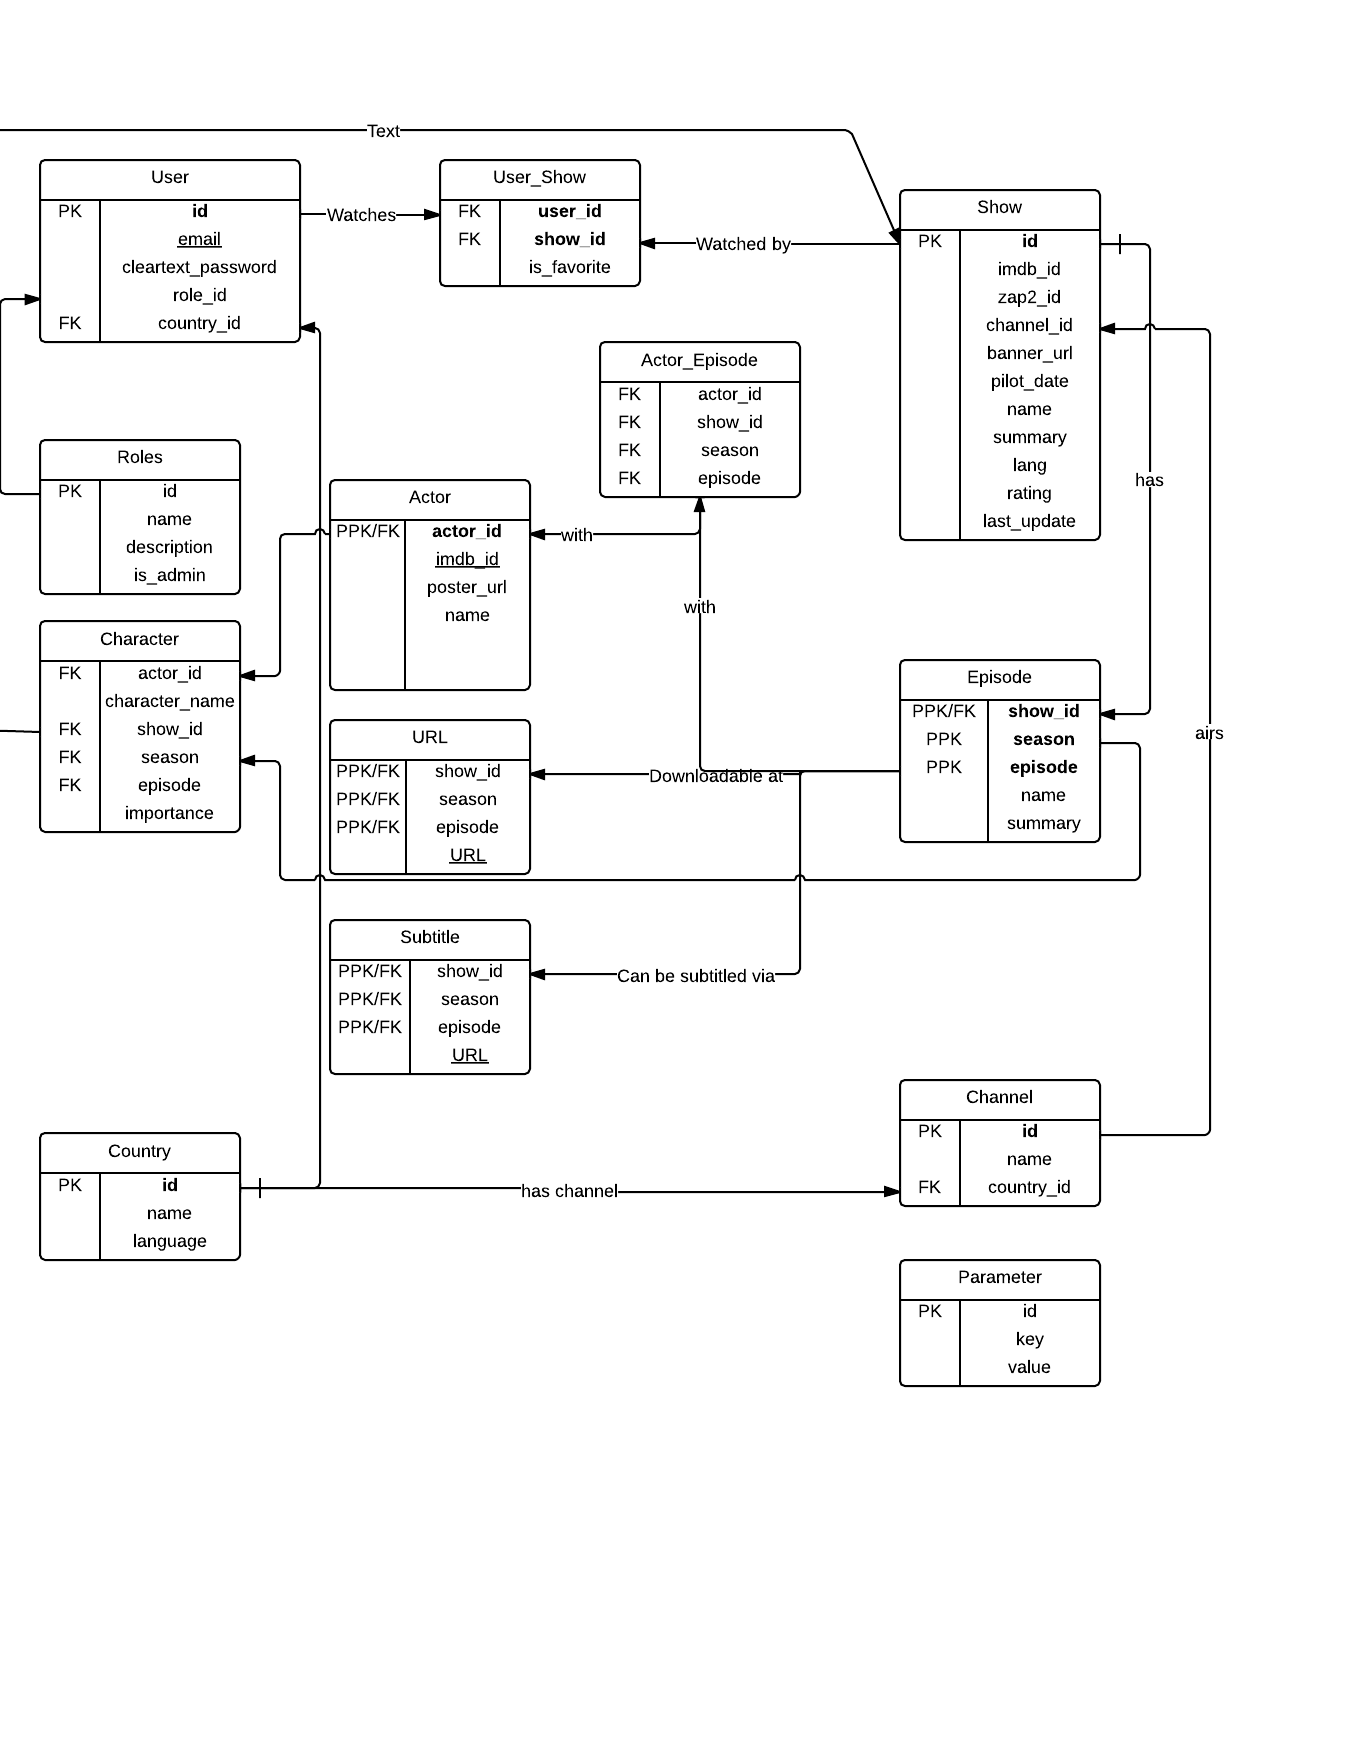
\includegraphics{erd}
\subsubsection{Entity-Relationship Diagram}



\subsection{Week 1}
The project startet off with a meeting. After about two hours of brainstorming we had a couple of ideas of what we could do. We then gave ourself until the next day to think about the alternatives. \\
The next day we discussed wich of the ideas would be the most appropriate for our combined skill level and the time we had. After a little while, we came to the conclusion that making a website that holds information about tv-shows would be both challenching and interesting.\\

The rest of the week was spent on casually brainstorming ideas about the website and writing them down.
...
\subsection{Week 2}

The beginning of week 2 on spent on discussing exactly what kind of functionality we wanted and what tasks that had to be done, and in what order.
After we had a clear overview about what had to done, we started laying out a plan on how we would share the task between eachother.
...
\subsection{Week 3}
At this point we felt like we had done enough planning and was quite ready to start coding. Each of us had our tasks and worked on those task seperatly for about a week to get the most essential building stones up and running.\\
...
\subsection{Week 4}
when most of the fundemental part where done we could start coding functionality. A lot of time was spent on including a functionality and then adapting the rest of the code to work with the functionality through a lot of bug testing. We had a list of functions we wanted to implement, so we picked at will what we wanted to do. When we where done with one task, we picked another one.
...
\subsection{Week 5}
Week 5 were mostly spent on finishing up as many functions as we could manage, fixing as many bugs as we could and make the code as efficient as possible.\\

\textbf{An overview over who had the most to do with most of the files:}\\

\begin{tabular}{| l | l | l | l |}
\hline
Tommy 				& Halvor 			& Victor\\ \hline
configurationClass.php		& tvdbClass.php		& activeRecord.php \\
databaseClass.php 			& fileHandlerClass.php 	& channelClass.php \\
index.php				&emailSenderClass.php 	& episodeClass.php\\
userClass.php 			&				& showClass.php\\
userResetPasswordClass.php 	&				& table.php\\
tpbClass.php 			&				& browse.php\\
 					&				& details.php\\						
\hline
\end{tabular}

\end{document}
